%\graphicspath{{~/Pictures/Screenshots/}}
\graphicspath{{./img}}
\section*{\LARGE{Цель практической работы}}
\addcontentsline{toc}{section}{Цель практической работы}
Создать примеры, реализующие основные элементы управления:

\begin{itemize}
	\item Элемент TextView и его атрибуты. Установка элемента в коде.
		Используя атрибут android:autoLink вывести на экран ссылку и телефон;
	\item Элемент EditText и его атрибуты. Используя атрибуты
		android:hint и android:inputType задать текст, который будет
		отображаться в качестве подсказки, если элемент EditText пуст
		и клавиатуру для ввода. Реализовать два поля.
		Первое поле --- однострочное, а второе --- многострочное.
		Введенные символы в первом поле --- отображаются во втором;
	\item Элемент Button и его атрибуты. Реализовать на экране кнопку с
		надписью “Ввод”. После нажатия на кнопку выводится текст из первого
		поля во второе. Реализовать аналогичный пример полностью в коде;
	\item Класс Toast. Всплывающие окна. Toast можно использовать
		только в коде java. Реализуйте это, используя метод Toast.makeText().
		В качестве времени показа окна можете использовать целочисленное
		значение - колическо миллисекунд или встроенные константы
		\verb|Toast.LENGTH_LONG| (2000 миллисекунд)
		и \verb|Toast.LENGTH_SHORT| (2000 миллисекунд).
		Используйте метод setGravity для указания, в какой части
		контейнера надо позиционировать Toast;
	\item Элемент Snackbar. Реализуйте пример с помощью метода make().
		Прикрепление обработчика события. Реализуйте пример с помощью метода
		setAction().Реализуйте пример с настройкой визуального вида;
	\item Элементы Checkbox. Реализуйте пример с несколькими
		флажками которые могут находиться в отмеченном и неотмеченном
		состоянии;
	\item Слушатель OnCheckedChangeListener. Реализуйте пример с
		помощью метода onCheckedChanged;
	\item Элемент ToggleButton. Реализуйте пример с помощью атрибутов
		android:textOn и android:textOff. Реализуйте пример создания элемента
		ToggleButton в коде java;
	\item Класс RadioButton Реализуйте пример;
	\item Элемент DatePicker. Реализуйте пример;
	\item Элемент TimePicker Реализуйте пример;
	\item Элемент SeekBar (Ползунок). Реализуйте пример.
\end{itemize}

\clearpage

\section*{\LARGE{Выполнение практической работы}}
\addcontentsline{toc}{section}{Выполнение практической работы}

\section{Элемент TextView}
Для простого вывода текста на экран предназначен элемент TextView. 
Он просто отображает текст без возможности его редактирования. 
Некоторые его основные атрибуты:

\begin{itemize}
	\item \texttt{android:text}: устанавливает текст элемента;
	\item \texttt{android:textSize}: устанавливает высоту текста,
		в качестве единиц измерения для указания высоты используются sp;
	\item \texttt{android:background}: задает фоновый цвет элемента в виде
		цвета в шестнадцатиричной записи или в виде цветового ресурса;
	\item \texttt{android:textColor}: задает цвет текста;
	\item \texttt{android:textAllCaps}: при значении true делает все символы
		в тексте заглавными;
	\item \texttt{android:textDirection}: устанавливает направление текста.
		По умолчанию используется направление слева направо, но с помощью
		значения rtl можно установить направление справо налево;
	\item \texttt{android:textAlignment}: задает выравнивание текста;
	\item \texttt{ndroid:fontFamily}: устанавливает тип шрифта.
\end{itemize}

Чтобы вывести на экран какую-нибудь ссылку,
по нажатию на которые производилось бы определенное действие,
используется атрибут \texttt{android:autoLink}
Данный виджет проиллюстрирован на листинге~\ref{lst:TextView}.
\begin{lstlisting}[language=xml, caption=\leftline{xml}, label=lst:TextView]
<TextView
        android:id="@+id/Work5_1_textView"
        android:layout_width="0dp"
        android:layout_height="wrap_content"
        android:layout_margin="10dp"
        android:autoLink="web"

        android:background="@color/black"
        android:text="https://english.mirea.ru"

        android:textAllCaps="true"
        android:textColor="@color/white"
        android:textSize="20sp"
        app:layout_constraintBottom_toBottomOf="parent"
        app:layout_constraintLeft_toLeftOf="parent"
        app:layout_constraintRight_toRightOf="parent"
        app:layout_constraintTop_toTopOf="parent" />
\end{lstlisting}
\img{png1}{TextView}


\section{Элемент EditText}
Элемент EditText является подклассом класса TextView. Он также 
представляет текстовое поле, но теперь уже с возможностью ввода и 
редактирования текста. Таким образом, в EditText мы можем использовать 
все те же возможности, что и в TextView. Из тех атрибутов, что не 
рассматривались в теме про TextView, следует отметить атрибут android:hint. 
Он позволяет задать текст, который будет отображаться в качестве 
подсказки, если элемент EditText пуст. Кроме того, мы можем использовать 
атрибут \texttt{android:inputType}, который позволяет задать
клавиатуру для ввода.
Данный виджет проиллюстрирован на листинге~\ref{lst:EditTextXML}.
\begin{lstlisting}[language=xml, caption=\leftline{EditTextXML}, label=lst:EditTextXML]
<EditText
	android:id="@+id/f_input"
	android:layout_width="wrap_content"
	android:layout_height="wrap_content"
	android:layout_weight="1"
	android:ems="10"
	android:hint="first message"
	android:inputType="text"
	android:textSize="25sp"

	app:layout_constraintLeft_toLeftOf="parent"
	app:layout_constraintRight_toRightOf="parent"
	app:layout_constraintTop_toTopOf="parent" />

<EditText
	android:id="@+id/s_input"
	android:layout_width="wrap_content"
	android:layout_height="wrap_content"
	android:layout_weight="1"
	android:ems="10"
	android:hint="Second message"
	android:inputType="textMultiLine"
	android:textSize="25sp"
	android:editable="true"

	app:layout_constraintLeft_toLeftOf="parent"
	app:layout_constraintRight_toRightOf="parent"
	app:layout_constraintTop_toBottomOf="@+id/f_input" />
\end{lstlisting}
\begin{lstlisting}[language=Kotlin, caption=\leftline{EditTextKotlin}, label=lst:EditTextKotlin]
override fun onCreate(savedInstanceState: Bundle?) {
        super.onCreate(savedInstanceState)
        setContentView(R.layout.activity_work52)
        val editText = findViewById<EditText>(R.id.f_input)

        editText.addTextChangedListener(object : TextWatcher {
            override fun afterTextChanged(s: Editable) {}
            override fun beforeTextChanged(
                s: CharSequence, start: Int,
                count: Int, after: Int
            ) {
            }

            override fun onTextChanged(s: CharSequence, start: Int, before: Int, count: Int) {
                val editTextF = findViewById<EditText>(R.id.f_input)
                val editTextS = findViewById<EditText>(R.id.s_input)
                val text = editTextS.text
                text.replace(0, text.length, editTextF.text)
                editTextS.setText(text)
            }
        })
    }
\end{lstlisting}
\img{png2}{EditText}


\section{Элемент Button}
Одним из часто используемых элементов являются кнопки, которые 
представлены классом android.widget.Button. Ключевой особенностью кнопок 
является возможность взаимодействия с пользователем через нажатия. 
Наследуется от класса TextView с новым методом \texttt{onClick}.
Данный виджет проиллюстрирован на листинге~\ref{lst:button}.
\begin{lstlisting}[language=xml, caption=\leftline{buttonXml}, label=lst:button]
<TextView
        android:id="@+id/textView"
        android:layout_width="0dp"
        android:layout_height="wrap_content"
        android:textSize="34sp"
        app:layout_constraintTop_toTopOf="parent"
        app:layout_constraintLeft_toLeftOf="parent"
        app:layout_constraintRight_toRightOf="parent"/>
    <EditText
        android:id="@+id/editText"
        android:layout_width="0dp"
        android:layout_height="wrap_content"
        android:hint="Введите имя"
        app:layout_constraintTop_toBottomOf="@+id/textView"
        app:layout_constraintLeft_toLeftOf="parent"
        app:layout_constraintRight_toRightOf="parent" />
    <Button
        android:layout_width="wrap_content"
        android:layout_height="wrap_content"
        android:text="Ввод"
        android:onClick="sendMessage"
        app:layout_constraintTop_toBottomOf="@+id/editText"
        app:layout_constraintLeft_toLeftOf="parent" />
\end{lstlisting}
\begin{lstlisting}[language=Kotlin, caption=\leftline{buttonXmlKotlin}, label=lst:buttonXmlKotlin]
override fun onCreate(savedInstanceState: Bundle?) {
        super.onCreate(savedInstanceState)
        setContentView(R.layout.activity_work53)
    }

    fun sendMessage(view: View?) {
        val textView = findViewById<TextView>(R.id.textView)
        val editText = findViewById<EditText>(R.id.editText)
        textView.text = "Добро пожаловать, " + editText.text
    }
\end{lstlisting}
\img{png3}{button}
\subsection{Элемент Button в коде}
Пример вышеуказанного задания в коде на листинге~\ref{lst:buttonKotlin}.

\begin{lstlisting}[language=Kotlin, caption=\leftline{buttonKotlin}, label=lst:buttonKotlin]
override fun onCreate(savedInstanceState: Bundle?) {
        super.onCreate(savedInstanceState)
        val constraintLayout = ConstraintLayout(this)

        val textView = TextView(this)
        textView.setId(View.generateViewId())
        val textViewLayout = ConstraintLayout.LayoutParams(
            ConstraintLayout.LayoutParams.MATCH_CONSTRAINT,
            ConstraintLayout.LayoutParams.WRAP_CONTENT
        )
        textViewLayout.topToTop = ConstraintLayout.LayoutParams.PARENT_ID
        textViewLayout.leftToLeft = ConstraintLayout.LayoutParams.PARENT_ID
        textViewLayout.rightToRight = ConstraintLayout.LayoutParams.PARENT_ID
        textView.setLayoutParams(textViewLayout)
        constraintLayout.addView(textView)

        val editText = EditText(this)
        editText.setId(View.generateViewId())
        editText.setHint("Введите имя")
        val editTextLayout = ConstraintLayout.LayoutParams(
            ConstraintLayout.LayoutParams.MATCH_CONSTRAINT,
            ConstraintLayout.LayoutParams.WRAP_CONTENT
        )
        editTextLayout.topToBottom = textView.getId()
        editTextLayout.leftToLeft = ConstraintLayout.LayoutParams.PARENT_ID
        editTextLayout.rightToRight = ConstraintLayout.LayoutParams.PARENT_ID
        editText.setLayoutParams(editTextLayout)
        constraintLayout.addView(editText)

        val button = Button(this)
        button.setText("Ввод")
        val buttonLayout = ConstraintLayout.LayoutParams(
            ConstraintLayout.LayoutParams.WRAP_CONTENT, ConstraintLayout.LayoutParams.WRAP_CONTENT
        )
        buttonLayout.topToBottom = editText.getId()
        buttonLayout.leftToLeft = ConstraintLayout.LayoutParams.PARENT_ID
        button.setLayoutParams(buttonLayout)
        constraintLayout.addView(button)

        button.setOnClickListener(object : View.OnClickListener {
            override fun onClick(v: View?) {
                textView.setText("Добро пожаловать, " + editText.getText())
            }
        })

        setContentView(constraintLayout)
    }
\end{lstlisting}



\section{Класс Toast}
Для создания простых уведомлений в Android используется класс 
Toast. Фактически Toast представляет всплывающее окно с некоторым 
текстом, которое отображается в течение некоторого времени. Объект Toast 
нельзя создать в коде разметки xml, например, в файлe activity\_main.xml. 
Toast можно использовать только в коде.
Данный виджет проиллюстрирован на листинге~\ref{lst:toast}.

\begin{lstlisting}[language=Kotlin, caption=\leftline{toast}, label=lst:toast]
fun onClick(view: View?) {
        val toast = Toast.makeText(this, "Hello Android!", Toast.LENGTH_LONG)
        toast.show()
    }
\end{lstlisting}
\img{png4}{Toast}

\section{Элемент Snackbar}
Элемент Snackbar в некотором роде похож на Toast: он также позволяет 
выводить всплывающие сообщения, но теперь сообщения растягиваются по 
ширине экрана.

\subsection{C помощью метода make()}
Вызов виджета с помощью метода make() проиллюстрирован на листинге~\ref{lst:snackbarmake}.
\begin{lstlisting}[language=Kotlin, caption=\leftline{snackbar}, label=lst:snackbarmake]
fun onClick(view: View?) {
        if (view != null) {
            Snackbar.make(view, "Hello Android", Snackbar.LENGTH_LONG)
                .show()
        }
    }
\end{lstlisting}
\subsection{Прикрепление обработчика события}
Snackbar позволяет добавить виджету действие, чтобы пользователь мог как-то прореагировать на сообщение.
Например, изменим код MainActivity следующим образом:
\begin{lstlisting}[language=Kotlin, caption=\leftline{setAction}, label=lst:setAction]
fun onClick(view: View?) {
        val snackbar = view?.let { Snackbar.make(it, "Hello Android", Snackbar.LENGTH_LONG) }
        snackbar?.setTextColor(CYAN)
        snackbar?.setBackgroundTint(GRAY)
        snackbar?.setActionTextColor(MAGENTA)
        snackbar?.setAction("Next...", View.OnClickListener {
            val toast = Toast.makeText(applicationContext, "Next clicked!", Toast.LENGTH_LONG)
            toast.show()
        })
        snackbar?.show()
    }
\end{lstlisting}
\img{png5}{setAction}
\section{Элементы Checkbox}
Элементы Checkbox представляют собой флажки, которые могут 
находиться в отмеченном и неотмеченном состоянии.
Флажки позволяют производить множественный выбор из нескольких значений.
Данный виджет проиллюстрирован на листинге~\ref{lst:checkbox}.

\begin{lstlisting}[language=xml, caption=\leftline{checkbox}, label=lst:checkbox]
<TextView android:id="@+id/selection"
        android:layout_width="wrap_content"
        android:layout_height="wrap_content"
        android:textSize="26sp"
        app:layout_constraintLeft_toLeftOf="parent"
        app:layout_constraintTop_toTopOf="parent"/>

    <CheckBox android:id="@+id/java"
        android:layout_width="wrap_content"
        android:layout_height="wrap_content"
        android:text="Java"
        android:textSize="26sp"

        android:onClick="onCheckboxClicked"

        app:layout_constraintLeft_toLeftOf="parent"
        app:layout_constraintTop_toBottomOf="@+id/selection"/>

    <CheckBox android:id="@+id/kotlin"
        android:layout_width="wrap_content"
        android:layout_height="wrap_content"
        android:text="Kotlin"
        android:textSize="26sp"

        android:onClick="onCheckboxClicked"

        app:layout_constraintLeft_toLeftOf="parent"
        app:layout_constraintTop_toBottomOf="@+id/java"/>
\end{lstlisting}

\begin{lstlisting}[language=Kotlin, caption=\leftline{checkbox Kotlin}, label=lst:checkboxKotlin]
fun onCheckboxClicked(view: View) {
        val language = view as CheckBox
        if (language.text !in checkedBoxes && language.isChecked){
            checkedBoxes.add(language.text as String)
        } else if(language.text in checkedBoxes && !language.isChecked) {
            checkedBoxes.remove(language.text as String)
        }


        var str = ""
        for ( i in checkedBoxes){
            str += "$i "
        }

        val selection = findViewById<TextView>(R.id.selection)
        selection.text = str
    }
\end{lstlisting}
\img{png6}{checkbox}

\section{Слушатель OnCheckedChangeListener}
Применение слушателя OnCheckedChangeListener представляет
альтернативный способ отслеживания изменения флажка. Этот слушатель 
срабатывает, когда устанавливается или убирается отметка на флажке.\par
Слушатель OnCheckedChangeListener определен в базовом классе
CompoundButton и определяет один метод --- \texttt{onCheckedChanged}. Первый
параметр этого метода \texttt{buttonView} --- сам измененный флажок CheckBox.
А второй параметр \texttt{isChecked} указывает, отмечен ли флажок.
Данный виджет проиллюстрирован на листинге~\ref{lst:OnCheckedChangeListener}.

\begin{lstlisting}[language=Kotlin, caption=\leftline{OnCheckedChangeListener Kotlin}, label=lst:OnCheckedChangeListener]
private val checkedBoxes : ArrayList<String> = arrayListOf()

    override fun onCreate(savedInstanceState: Bundle?) {
        super.onCreate(savedInstanceState)
        setContentView(R.layout.activity_work59)

        val enableJavaBox = findViewById<CheckBox>(R.id.java)
        enableJavaBox.setOnCheckedChangeListener{buttonView, isChecked ->
            onCheckedChanged(buttonView, isChecked)}

        val enableKotlinBox = findViewById<CheckBox>(R.id.kotlin)
        enableKotlinBox.setOnCheckedChangeListener{buttonView, isChecked ->
            onCheckedChanged(buttonView, isChecked)}
    }

    private fun onCheckedChanged(buttonView: CompoundButton?, isChecked: Boolean) {
        if (buttonView != null) {
            if (buttonView.text !in checkedBoxes && isChecked){
                checkedBoxes.add(buttonView.text as String)
            } else if(buttonView.text in checkedBoxes && !isChecked) {
                checkedBoxes.remove(buttonView.text as String)
            }

        var str = ""
        for ( i in checkedBoxes){
            str += "$i "
        }

        val selection = findViewById<TextView>(R.id.selection)
        selection.text = str
        }
    }
\end{lstlisting}

\section{Элемент ToggleButton}
ToggleButton подобно элементу CheckBox может пребывать в двух 
состояниях: отмеченном и неотмеченном, причем для каждого состояния мы 
можем отдельно установить свой текст.
Данный виджет проиллюстрирован на листинге~\ref{lst:ToggleButton}.

\begin{lstlisting}[language=xml, caption=\leftline{ToggleButton XML}, label=lst:ToggleButton]
<ToggleButton
        android:id="@+id/toggle"
        android:layout_width="wrap_content"
        android:layout_height="wrap_content"
        android:textOn="Ligth on"
        android:textOff="Ligth off"
        android:onClick="onToggleClicked"
        app:layout_constraintLeft_toLeftOf="parent"
        app:layout_constraintTop_toTopOf="parent" />
\end{lstlisting}

\begin{lstlisting}[language=Kotlin, caption=\leftline{ToggleButton Kotlin}, label=lst:ToggleButtonKotlin]
fun onToggleClicked(view: View) {

        val on = (view as ToggleButton).isChecked
        if (on) {
            Toast.makeText(this, "Ligth on", Toast.LENGTH_LONG).show()
            view.setBackgroundColor(WHITE)
        } else {
            Toast.makeText(this, "Ligth off!", Toast.LENGTH_LONG).show()
            view.setBackgroundColor(BLACK)
        }
    }
\end{lstlisting}
\img{png7}{ToggleButton}




\subsection{ToggleButton в коде}
Создание элемента ToggleButton в коде:
\begin{lstlisting}[language=Kotlin, caption=\leftline{ToggleButton Kotlin}, label=lst:ToggleButtoninKotlin]
override fun onCreate(savedInstanceState: Bundle?) {
        super.onCreate(savedInstanceState)
        val layout = ConstraintLayout(this)
        val layoutParams = ConstraintLayout.LayoutParams(
            ConstraintLayout.LayoutParams.WRAP_CONTENT,
            ConstraintLayout.LayoutParams.WRAP_CONTENT
        )
        val toggleButton = ToggleButton(this)
        toggleButton.textOff = "Выключено"
        toggleButton.textOn = "Включено"
        toggleButton.text = "Выключено"
        toggleButton.setOnClickListener { view ->
            val on = (view as ToggleButton).isChecked
            if (on) {
                Toast.makeText(applicationContext, "Свет включен", Toast.LENGTH_LONG).show()
                view.setBackgroundColor(Color.WHITE)
            } else {
                Toast.makeText(applicationContext, "Свет выключен!", Toast.LENGTH_LONG).show()
                view.setBackgroundColor(Color.GRAY)
            }
        }
        layoutParams.leftToLeft = ConstraintLayout.LayoutParams.PARENT_ID
        layoutParams.topToTop = ConstraintLayout.LayoutParams.PARENT_ID
        layout.addView(toggleButton)
        setContentView(layout)
    }
\end{lstlisting}
\section{Класс RadioButton}
Схожую с флажками функциональность предоставляют 
переключатели, которые представлены классом RadioButton. Но в отличие от 
флажков единовременно в группе переключателей мы можем выбрать только 
один переключатель. Чтобы создать список переключателей для выбора, 
вначале надо создать объект RadioGroup, который будет включать в себя все 
переключатели.
Данный виджет проиллюстрирован на листинге~\ref{lst:RadioGroup}.
\begin{lstlisting}[language=xml, caption=\leftline{RadioGroup XML}, label=lst:RadioGroup]
<TextView android:id="@+id/selection"
        android:layout_width="wrap_content"
        android:layout_height="wrap_content"
        android:textSize="26sp"
        app:layout_constraintLeft_toLeftOf="parent"
        app:layout_constraintTop_toTopOf="parent"/>

    <RadioGroup
        android:id="@+id/radios"
        android:layout_width="match_parent"
        android:layout_height="wrap_content"
        android:orientation="vertical"
        app:layout_constraintLeft_toLeftOf="parent"
        app:layout_constraintTop_toBottomOf="@+id/selection"
        >

        <RadioButton android:id="@+id/java"
            android:layout_width="wrap_content"
            android:layout_height="wrap_content"
            android:text="Java"
            android:onClick="onRadioButtonClicked"/>
        <RadioButton android:id="@+id/kotlin"
            android:layout_width="wrap_content"
            android:layout_height="wrap_content"
            android:text="Kotlin"
            android:onClick="onRadioButtonClicked"/>
    </RadioGroup>
\end{lstlisting}

\begin{lstlisting}[language=Kotlin, caption=\leftline{RadioGroup Kotlin}, label=lst:RadioGroupKotlin]
fun onRadioButtonClicked(view: View) {
        val checked = (view as RadioButton).isChecked
        val selection = findViewById<TextView>(R.id.selection)
        when (view.getId()) {
            R.id.java -> if (checked) {
                selection.text = "Java"
            }
            R.id.kotlin -> if (checked) {
                selection.text = "Kotlin"
            }
        }
    }
\end{lstlisting}
\img{png8}{RadioGroup}

\section{Элемент DatePicker}

DatePicker представляет элемент для выбора даты. Среди его атрибутов 
можно отметить следующие:
\begin{itemize}
	\item \texttt{android:calendarTextColor}: цвет текста календаря;
	\item \texttt{android:calendarViewShown}: указывает, будет ли
		отображаться вид календаря;
	\item \texttt{android:datePickerMode}: устанавливает режим выбора даты;
	\item \texttt{android:dayOfWeekBackground}: устанавливает фоновый цвет
		панели выбора дня недели;
	\item \texttt{android:endYear}: устанавливает последний отображаемый год;
	\item \texttt{android:firstDayOfWeek}: устанавливает первый день недели;
	\item \texttt{android:headerBackground}: устанавливает фоновый цвет
		для панели выбранной даты;
	\item \texttt{android:maxDate}: устанавливает максимальную отображаемую
		дату в формате mm/dd/yyyy;
	\item \texttt{android:minDate}: устанавливает минимальную отображаемую
		дату в формате mm/dd/yyyy;
	\item \texttt{android:spinnersShown}: указывает, будет ли отображаться
		спиннер в виджете;
	\item \texttt{android:startYear}: устанавливает начальный
		отображаемый год;
	\item \texttt{android:yearListSelectorColor}: устанавливает цвет для
		поля выбора года.
\end{itemize}

Данный виджет проиллюстрирован на рисунке~\ref{fig:datepicker}.

\begin{image}
	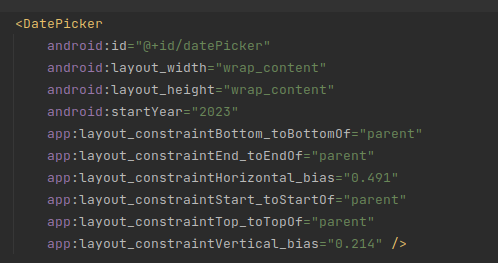
\includegraphics[width=0.8\textwidth]{Screenshot from 2023-03-25 18-07-26.png}
	\caption{Пример использования DatePicker}
	\label{fig:datepicker}
\end{image}

\section{Элемент TimePicker}
TimePicker представляет виджет для выбора времени, который может 
отображать время либо в 24-часовом, либо в 12-часовом формате. Среди 
атрибутов TimePicker следует выделить \texttt{timePickerMode},
который позволяет режим отображения и может принимать одно из двух значений:
\texttt{clock} (отображение в виде часов) и
\texttt{spinner} (отображение в виде спиннера).
Среди методов TimePicker можно отметить следующие:

\begin{itemize}
	\item \texttt{int getHour()}: возвращает час (в 24-часом формате);
	\item \texttt{int getMinute()}: возвращает минуты;
	\item \texttt{boolean is24HourView()}: возвращает true, если
		используется 24- часовой формат;
	\item \texttt{void setHour(int hour)}: устанавливает час для TimePicker;
	\item \texttt{void setIs24HourView(Boolean is24HourView)}:
		устанавливает 24- часовой формат;
	\item \texttt{void setMinute(int minute)}: устанавливает минуты;
	\item \texttt{void setOnTimeChangedListener(TimePicker.OnTimeChangedListener 
		onTimeChangedListener)}: устанавливает слушатель изменения времени 
		в TimePicker в виде объекта.
\end{itemize}

Данный виджет проиллюстрирован на рисунке~\ref{fig:timepicker}.

\begin{image}
	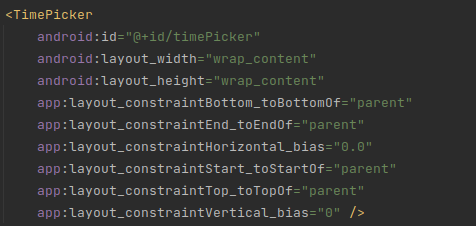
\includegraphics[width=0.8\textwidth]{Screenshot from 2023-03-25 18-09-56.png}
	\caption{Пример использования TimePicker}
	\label{fig:timepicker}
\end{image}

\section{Элемент SeekBar (Ползунок)}
Элемент SeekBar выполняет роль ползунка, то есть шкалу делений, на 
которой мы можем менять текущую отметку. Среди его атрибутов можно 
отметить следующие:

\begin{itemize}
	\item \texttt{android:max}: устанавливает максимальное значение;
	\item \texttt{android:min}: устанавливает минимальное значение;
	\item \texttt{android:progress}: устанавливает текущее значение,
		которое находится в диапазоне между минимальным и максимальным.
\end{itemize}

Данный виджет проиллюстрирован на рисунке~\ref{fig:seekbar}.

\begin{image}
	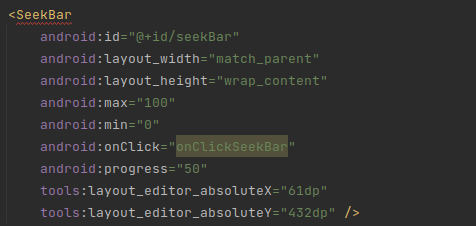
\includegraphics[width=0.8\textwidth]{Screenshot from 2023-03-25 18-11-54.png}
	\caption{Пример использования SeekBar}
	\label{fig:seekbar}
\end{image}


\clearpage

\section*{\LARGE{Вывод}}
\addcontentsline{toc}{section}{Вывод}
В ходе проделанной практической работы были получены навыки и 
знания с работой TextView, EditView, Button, Toast, Snackbar, CheckBox, 
ToggleButton, RadioButton/RadioGroup, TimePicker, DatePicker, Seekbar.

